\documentclass[11pt]{beamer}
\usepackage[utf8]{inputenc}
\usepackage[T1]{fontenc}
\usepackage[french]{babel}
\usepackage{amsmath}
\usepackage{amsfonts}
\usepackage{amssymb}
\usepackage{graphicx}
\usepackage{siunitx}

\usetheme{Pittsburgh}

\usefonttheme{serif}

\begin{document}
	\author{Laura Guislain \and Nicolas Lecoeur \and André Kalouguine}
	\title{Mouvement des E.coli autour de particules colloïdales}
	\subtitle{Et comparaison au mouvement brownien?}
	\titlegraphic{\includegraphics[height=1cm]{logo_ens}}
	\institute{E.N.S. de Lyon}
	%\date{}
	\subject{Characterization du mouvement bactérien et comparaison au mouvement brownien.}
	%\setbeamercovered{transparent}
	\setbeamertemplate{footline}{\hspace{0.5em}\insertframenumber}
	\setbeamertemplate{navigation symbols}{}
	\setbeamertemplate{caption}[numbered]
	\addtobeamertemplate{footline}{\vspace{-0.5em}}{\vspace{0.5em}}
\begin{frame}[plain]
	\maketitle
\end{frame}
\addtocounter{framenumber}{-1}

%\frame{\tableofcontents}

\section{Méthode experimentale}

\begin{frame}{Cellules d'observation}
\begin{columns}
	\column{0.5\linewidth}
	\begin{figure}
		\centering
		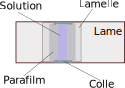
\includegraphics[width=\linewidth]{Cellule1}
		\caption{Premier modèle de cellule}
		\label{fig:cellule1}
	\end{figure}
	
	\column{0.5\linewidth}
	\begin{figure}
	\centering
	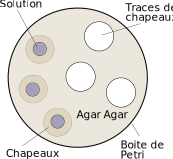
\includegraphics[width=\linewidth]{Cellule2}
	\caption{Second modèle de cellule}
	\label{fig:cellule2}
	\end{figure}
\end{columns}
\end{frame}

\begin{frame}{Microscope et caméra}
	Du blabla sur la fluorescence, mettre une photo du microscope
\end{frame}

\section{Étude préliminaire du mouvement en milieu simple}


\subsection{Mouvement brownien de colloïdes petits}
\begin{frame}{Mouvement brownien}
\framesubtitle{Observation du mouvement}
	\begin{figure}
		\centering
		\includegraphics[width=0.9\linewidth]{Trajectory_brownian}
		\caption{Trajectoire d'un colloïde suivi sur \num{4e3} points}
		\label{fig:trajectory_b}
	\end{figure}
\end{frame}

\begin{frame}{Mouvement brownien}
\framesubtitle{Corrélation}
	\begin{figure}
		\centering
		\includegraphics[width=0.9\linewidth]{Correlation_brownian}
		\caption{La particule "oublie" ce qu'elle vient de faire très vite}
		\label{fig:correl_b}
	\end{figure}
\end{frame}

\begin{frame}{Mouvement brownien}
\framesubtitle{Statistique du mouvement}
\begin{figure}
	\centering
	\includegraphics[width=0.9\linewidth]{StatDepl_brownian}
	\caption{Répartition du déplacement selon x et y pour un colloïde}
	\label{fig:statdeplbrownian}
\end{figure}

\end{frame}


\begin{frame}{Mouvement brownien}
\framesubtitle{Coefficient de diffusion}
	content...
\end{frame}

\begin{frame}{Hermiticité de nos cellules}
Faire un graphique avec + de cellules.
\begin{figure}
	\centering
	\includegraphics[width=0.8\linewidth]{FuitesNico_1}
	\caption{Mouvement général des colloïdes dans une cellule. Si le module est proche de 1, alors $\mu$ comparabale devant $\sigma$}
	\label{fig:fuitesnico1}
\end{figure}

\end{frame}

\subsection{Mouvement des bactéries vivantes}
\begin{frame}{Mouvement bactérien}
	content...
\end{frame}

\section{Étude du mouvement autour de colloïdes ou qqch d'autre}

\end{document}